\documentclass[11pt]{article}
\usepackage[a4paper,margin=1in]{geometry}
\usepackage{amsmath,amssymb}
\usepackage{graphicx}
\usepackage{booktabs}
\usepackage{caption}
\usepackage{subcaption}
\usepackage{float}
\usepackage{xcolor}
\usepackage[hidelinks]{hyperref}
\usepackage{enumitem}
\usepackage{parskip}
\title{\textbf{Digital Image Processing --- Assignment 2}\\[0.3em]\large Problem 6: Motion Blur and Deblurring}
\author{Ujjwal Gupta}
\date{\today}
\begin{document}
\maketitle
\tableofcontents
\vspace{1em}

\section{Introduction / Problem Statement}

Problem 6 of the assignment (worth 20 of the 100 total points, the largest single problem) asks
for a full treatment of linear motion blur and its removal: modelling the blur, understanding
why its naive inversion fails, regularizing that inversion via Wiener deconvolution, and finally
applying the whole pipeline to a genuine self-captured blurred photograph. The official problem
statement is reproduced faithfully below (assignment PDF, pages 9--10), split into its four
required parts.

\textbf{6.1 Model and synthesize (5 pts).} For uniform linear motion of length $L$ pixels and
direction $\theta$, derive the continuous point spread function
\[
h(x,y)=\frac1L\int_{-L/2}^{L/2}\delta(x-t\cos\theta,\,y-t\sin\theta)\,dt,
\]
describe its discretization and normalization, state and consistently use a boundary convention
(circular recommended) for both forward blurring and deconvolution, blur the clean
instructor-provided image and add zero-mean Gaussian noise at a stated SNR (defined explicitly,
e.g.\ $\mathrm{SNR}_{\mathrm{dB}}=10\log_{10}\frac{\sum_{x,y,c}f(x,y,c)^2}{\sum_{x,y,c}n(x,y,c)^2}$,
not clipped before filtering), derive the motion OTF
$H(f_x,f_y)=\operatorname{sinc}\!\big(L(f_x\cos\theta+f_y\sin\theta)\big)$, and show that its
zero lines satisfy $f_x\cos\theta+f_y\sin\theta=m/L,\ m\in\mathbb Z\setminus\{0\}$, spaced $1/L$
apart and perpendicular to the motion direction.

\textbf{6.2 Naive inverse filtering and why it fails (5 pts).} Implement $\hat F=G/H$ for the
known synthetic blur, state the numerical floor used, show log-magnitude spectra of $G$ and the
raw (pre-clip) inverse estimate with the predicted OTF zeros marked, explain the noise
amplification there, and state in one sentence why any nonzero noise can become arbitrarily
large as $|H(u,v)|\to0$.

\textbf{6.3 Wiener deconvolution (5 pts).} Derive and implement the scalar-$K$ regularized
Wiener deconvolution filter
$\hat F(u,v)=\dfrac{H^*(u,v)G(u,v)}{|H(u,v)|^2+K}$, state the image scaling and interpretation
of $K$ as a constant noise-to-signal power ratio, sweep $K$ logarithmically, show low-$K$
inverse-filter failure and high-$K$ under-deconvolution, and report the PSNR-optimal $K$ at
$\ge3$ noise levels.

\textbf{6.4 Estimate the blur, then remove it (5 pts).} For a genuinely self-captured
motion-blurred photograph, estimate blur direction and approximate length from its
log-magnitude spectrum, build the estimated PSF, Wiener-deconvolve, report $\theta$, $L$, $K$,
and identify a visible artifact connected to a named limitation of the linear
spatially-invariant model (camera rotation, changing subject velocity, occlusion, or clipped
highlights), evaluated qualitatively since no sharp ground truth exists.

This problem sits at the heart of classical image restoration: motion blur is one of the most
common, physically well-understood forms of image degradation, and unlike denoising (Problem 5)
the degrading operator $H$ here is often \emph{known or estimable}, which makes deconvolution —
attempting to invert a convolution rather than merely suppress noise — the central technical
challenge. The problem also directly demonstrates why a naive matrix/Fourier inverse is
numerically catastrophic whenever the forward operator has near-zero frequency response, and how
the same Wiener machinery derived for denoising in Problem 5 generalizes immediately to this
regularized-inversion setting.

\section{Theoretical Background}

\subsection{The linear motion-blur PSF as a line integral}

A camera or scene point imaged under uniform linear relative motion of total length $L$ pixels
at angle $\theta$ (measured in the image plane) is smeared along the line segment the motion
traces out. If the point starts at the origin, its instantaneous position at parameter $t$
(for $t$ ranging uniformly over $[-L/2, L/2]$, representing the exposure interval) is
$(t\cos\theta,\, t\sin\theta)$. The point spread function is therefore the time-average of a
Dirac impulse tracing this line,
\[
h(x,y) = \frac1L \int_{-L/2}^{L/2} \delta\big(x - t\cos\theta,\; y - t\sin\theta\big)\, dt,
\]
i.e.\ a unit-mass line segment of length $L$ through the origin at angle $\theta$. The leading
factor $1/L$ normalizes the PSF's total mass to $\iint h(x,y)\,dx\,dy = 1$: since each
infinitesimal element $\delta(\cdots)\,dt$ contributes mass $dt$, integrating $t$ over an
interval of length $L$ accumulates total mass $L$, so dividing by $L$ gives unit mass — the
physical requirement that blurring does not change the total energy/brightness of the image.

\textbf{Discretization.} In practice $h$ is rasterized onto the pixel grid by sampling $t$
finely (in this implementation, $20\times$ oversampled relative to $L$) over $[-L/2, L/2]$,
computing the continuous offset $(x,y) = (t\cos\theta, t\sin\theta)$ for each sample, rounding to
the nearest integer pixel offset, and accumulating a histogram count at that offset in an array
the same size as the image to be blurred; the array is then normalized so its entries sum to 1.
The kernel is placed with its origin at array index $(0,0)$ (via modular wraparound) rather than
centred in the middle of the array — the layout \texttt{numpy.fft.fft2} expects for circular
convolution via direct multiplication with its own DFT.

\subsection{The motion OTF and its zero geometry}

The optical transfer function (OTF) is the 2-D Fourier transform of $h(x,y)$. Because $h$ is
supported entirely on the 1-D line through the origin at angle $\theta$, its Fourier transform
depends on spatial frequency $(f_x,f_y)$ only through the projection of $(f_x,f_y)$ onto the
motion direction, $u' \equiv f_x\cos\theta + f_y\sin\theta$ (a standard projection-slice-type
argument: a function constant along a direction in one domain has a Fourier transform supported
on the orthogonal line in the dual domain, and conversely a function confined to a line has a
transform that only varies along the projection of frequency onto the line's own direction).
Along that projected coordinate, $h$ reduces to a 1-D unit-mass rectangular (boxcar) function of
width $L$ centred at the origin, whose 1-D Fourier transform is the normalized sinc function.
Hence
\[
H(f_x,f_y) = \operatorname{sinc}\!\big(L(f_x\cos\theta+f_y\sin\theta)\big),
\qquad \operatorname{sinc}(z) = \frac{\sin(\pi z)}{\pi z}.
\]

\textbf{Zero lines.} $\operatorname{sinc}(z)=0$ exactly when $z=m$ for nonzero integer $m$, so
\[
H(f_x,f_y) = 0 \iff L(f_x\cos\theta+f_y\sin\theta) = m \iff
f_x\cos\theta+f_y\sin\theta = \frac{m}{L}, \quad m\in\mathbb Z\setminus\{0\}.
\]
Each such equation is a straight line in the $(f_x,f_y)$ plane: it is a level set of the
directional-projection coordinate $f_x\cos\theta+f_y\sin\theta$, which is constant along the
direction perpendicular to $(\cos\theta,\sin\theta)$ and varies linearly along
$(\cos\theta,\sin\theta)$ itself. Consequently the family of zero lines is \emph{perpendicular}
to the motion direction, and adjacent zero lines (consecutive integers $m$) are spaced $1/L$
apart along the projection coordinate. Because a discrete FFT grid only samples
$(f_x,f_y)=(u/M,v/N)$ at integer $(u,v)$, it will in general land \emph{near}, not exactly at,
these continuous zero lines.

\subsection{The naive inverse filter and its instability}

Given the known blur, the most direct way to recover $F$ from $G=HF+N$ (in the frequency
domain, under circular convolution) is to divide:
\[
\hat F(u,v) = \frac{G(u,v)}{H(u,v)} = F(u,v) + \frac{N(u,v)}{H(u,v)}.
\]
This is exact and perfectly recovers $F$ \emph{only if there is no noise} ($N\equiv0$). With
any nonzero noise, the second term $N(u,v)/H(u,v)$ is a fixed, generically nonzero numerator
divided by a denominator that can become arbitrarily small (at and near the OTF's zero lines
derived above). As $|H(u,v)|\to 0$, this ratio diverges without bound, so even an
infinitesimally small amount of noise at a near-zero-$H$ frequency is amplified to an arbitrarily
large value in $\hat F$ — the naive inverse filter is therefore numerically unstable at
precisely the frequencies identified by the zero-line geometry of Section 2.2, and in practice a
numerical floor must be applied to $|H|$ before dividing to keep the estimate finite (at the
cost of leaving severe, spatially-correlated noise amplification in the result).

\subsection{Wiener deconvolution as a regularized inverse}

The instability above is resolved by returning to the MMSE derivation used for denoising
(Problem 5), specialized to the case of a \emph{known, deterministic} linear degradation $H$
rather than an unknown signal PSD. The observation model is $G=HF+N$, and we again seek a
linear estimator $\hat F = W G$ minimizing $E\big[|F-\hat F|^2\big]$ at each frequency. Writing
the error as
\[
F - \hat F = F - W(HF+N) = (1-WH)F - WN,
\]
and assuming $F$ and $N$ uncorrelated with power spectra $S_{ff}$, $S_{nn}$:
\[
E\big[|F-\hat F|^2\big] = |1-WH|^2 S_{ff} + |W|^2 S_{nn}.
\]
Minimizing over $W$ (now generally complex, since $H$ itself carries phase) gives the Wiener
deconvolution filter
\[
W(u,v) = \frac{H^*(u,v)\,S_{ff}(u,v)}{|H(u,v)|^2 S_{ff}(u,v) + S_{nn}(u,v)}
       = \frac{H^*(u,v)}{|H(u,v)|^2 + S_{nn}(u,v)/S_{ff}(u,v)}.
\]
Replacing the frequency-dependent ratio $S_{nn}(u,v)/S_{ff}(u,v)$ by a single constant scalar
$K$ (a simplifying choice — a constant noise-to-signal power ratio, rather than a full function
of frequency) gives the implemented filter
\[
\boxed{\hat F(u,v) = \frac{H^*(u,v)\,G(u,v)}{|H(u,v)|^2 + K}.}
\]
This is exactly the general Wiener result of Problem 5 ($W=S_{ff}/(S_{ff}+S_{nn})$) specialized
to a known deterministic blur, with $K$ playing the role of the noise-to-signal ratio. Two
limits recover the behaviour already anticipated qualitatively: as $K\to0$, $\hat F \to G/H$
(the unstable naive inverse, wherever $H\ne0$); as $K\to\infty$ (or wherever $|H|^2\ll K$),
$\hat F \to H^*G/K$, a scaled, heavily smoothed estimate that under-deconvolves and leaves
residual blur. $K$ therefore interpolates continuously between these two failure modes, and an
intermediate value balances noise amplification against residual blur — the classic
bias-variance trade-off made explicit through a single scalar.

\section{Inputs and Outputs}

\textbf{Synthetic experiments (Sections 6.1--6.3):} the same clean, instructor-provided RGB
reference image used in Problem 5 (\texttt{data/provided/problem5\_6/reference\_image.jpg},
$3072\times2048$), downsampled to $768\times512$ for tractability. Unlike Problems 1--5, this
problem is processed in \textbf{RGB}, not grayscale — a deliberate choice, since the PDF's own
SNR formula is written with an explicit colour-channel sum $\sum_{x,y,c}$, signalling colour
treatment is expected. The motion OTF is identical across channels (computed once per
$(\theta,L)$) and applied independently to each of R, G, B. The clean image is blurred with
$L=25$ px, $\theta=30^\circ$, and zero-mean Gaussian noise is added at a stated
$\mathrm{SNR}_{\mathrm{dB}}=30$ (solved for directly, giving $\sigma=3.982$), not clipped before
filtering.

\textbf{Real-blur case study (Section 6.4):} a genuinely self-captured motion-blurred
photograph, \texttt{data/own\_captures/motion\_blur.jpeg} — a hand swiped quickly in front of
the camera against an otherwise stationary desk scene (bottle, plant, figurines). This is a real
photograph, not a synthetic blur, and the blur parameters $(\theta,L)$ are \emph{estimated} from
the photograph's own log-magnitude spectrum rather than being known in advance.

\textbf{Outputs produced:}
\begin{itemize}
\item The rasterized PSF, clean image, blurred image, and blurred+noise image
(\texttt{results/6\_1\_psf\_and\_blur.png}).
\item Numerical verification of the closed-form OTF against the DFT of the rasterized kernel
(\texttt{results/6\_1\_otf\_comparison.png}, \texttt{results/6\_1\_result.json}).
\item The naive-inverse log-magnitude spectra with predicted OTF zero lines overlaid
(\texttt{results/6\_2\_naive\_inverse\_spectra.png}) and the resulting (display-clipped)
noise-dominated spatial image (\texttt{results/6\_2\_naive\_inverse\_image.png}).
\item A $K$-sweep PSNR curve at four SNR levels (\texttt{results/6\_3\_K\_sweep.png}) and
qualitative low-/mid-/high-$K$ outputs (\texttt{results/6\_3\_K\_qualitative.png}).
\item The real photo's log-magnitude spectrum with estimated stripe spacing marked
(\texttt{results/6\_4\_spectrum\_stripes.png}) and the resulting deblurred output
(\texttt{results/6\_4\_real\_deblur.png}), evaluated qualitatively.
\end{itemize}

\section{Methodology / Implementation Pipeline}

\textbf{Implementation.} The core motion-blur machinery lives in
\texttt{src/dip\_a2/motion\_blur.py}: \texttt{motion\_psf\_otf(shape, L, theta\_deg,
oversample)} rasterizes the PSF as described in Section 2.1 and returns its DFT;
\texttt{motion\_otf\_analytic(shape, L, theta\_deg)} evaluates the closed-form sinc OTF directly
on the DFT frequency grid for comparison; \texttt{add\_noise\_at\_snr(signal, snr\_db, rng)}
solves for the Gaussian $\sigma$ that achieves a stated SNR; \texttt{naive\_inverse\_filter(G, H,
floor)} implements $\hat F=G/H$ with a floor on $|H|$; \texttt{wiener\_deconvolve(G, H, K)}
implements the boxed filter above; and \texttt{estimate\_motion\_blur(image, n\_angles)}
implements the blind blur-parameter estimation used in Section 6.4. The driver script is
\texttt{problem6.py}.

\textbf{Boundary convention.} \textbf{Circular}, as the PDF recommends, used identically for
both forward blurring (image FFT multiplied by the kernel's OTF, then inverse FFT) and all
deconvolution operations (naive inverse, Wiener) — no zero-padding step is used in this problem
(unlike Problems 2--3, whose $P=2N$ zero-padding exists to avoid a linear-vs-circular mismatch
for a small spatial kernel convolved with a large image). Here the kernel and every
deconvolution step are all meant to exactly invert each other under the \emph{same} circular
model, so a single consistent native-resolution circular convention is simpler and exactly
self-consistent between the forward and inverse operations.

\textbf{Numerical floor (naive inverse).} Wherever $|H(u,v)| < 10^{-3}$, that frequency's
magnitude is replaced by the floor value (preserving $H$'s phase) before dividing, so the naive
estimate remains finite everywhere, at the cost of extreme (but bounded) amplification exactly
at those frequencies.

\textbf{$K$-sweep methodology (Section 6.3).} $K$ is swept logarithmically from $10^{-6}$ to
$1$ (25 points) at four SNR levels (10, 20, 30, 40 dB); at each SNR level, the $K$ that maximizes
PSNR against the clean reference is recorded as the optimum. This sweep is itself
oracle-informed (it uses the clean reference to pick $K$), which is appropriate here since the
section's explicit purpose is to characterize the sensitivity of the optimal $K$ to noise level,
not to claim a deployable blind estimator — that is the separate, harder task of Section 6.4.

\textbf{Blind blur estimation (Section 6.4).} \texttt{estimate\_motion\_blur} computes the
photo's own centred log-magnitude spectrum; for a sweep of candidate angles, it projects the
spectrum radially outward along that angle and scores how periodically the projected profile
dips (via the 1-D FFT power of the profile, excluding DC); the angle with the strongest periodic
dip pattern is taken as the dark-stripe orientation, and the motion direction is perpendicular to
that (the stripes themselves are perpendicular to the motion direction, directly from the
zero-line geometry of Section 2.2). The blur length $L$ is recovered from the dominant spacing
of the detected dips via the same $1/L$ relationship.

\textbf{Validation of correctness.} The closed-form analytic OTF was checked numerically against
the actual DFT of the rasterized spatial kernel: median $|\Delta H| = 0.0136$, 99th-percentile
$|\Delta H| = 0.3646$, maximum $|\Delta H| = 0.5400$ (occurring at frequency
$\approx(-0.289,-0.500)$, i.e.\ essentially exactly at the Nyquist frequency of the 768-pixel
axis — expected, since the rasterized kernel is a genuinely discrete, periodic signal subject to
aliasing, whereas the closed-form sinc assumes a continuous, unaliased projection, and the two
can only disagree substantially at the single most alias-prone frequency). Naive-inverse
amplification was quantified directly: mean $|\hat F|$ at floored bins ($|H|<10^{-3}$) was
$1.49\times10^6$ versus $7.26\times10^4$ at other high-frequency bins — a $20.5\times$ ratio,
confirming the predicted amplification at the OTF zero lines.

\section{Results and Discussion}

\subsection{PSF, blur synthesis, and OTF verification}

\begin{figure}[H]
\centering
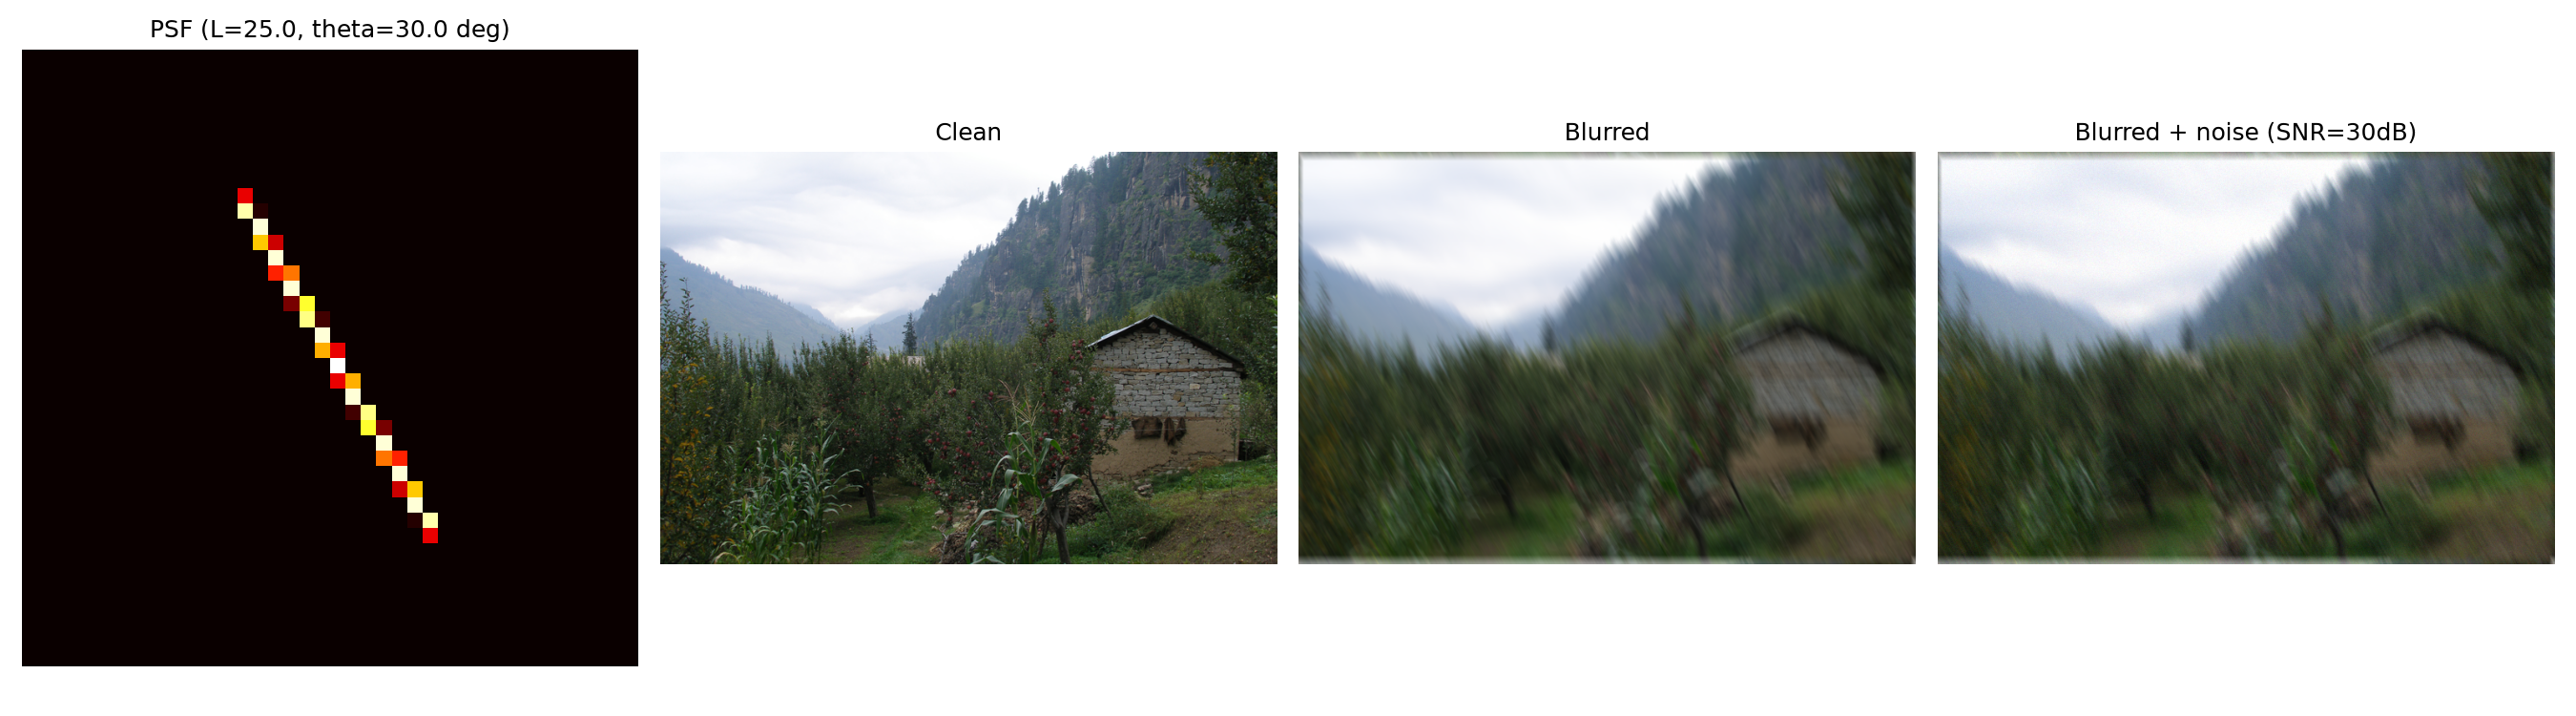
\includegraphics[width=0.8\linewidth]{results/6_1_psf_and_blur.png}
\caption{Rasterized motion PSF ($L{=}25$px, $\theta{=}30^\circ$), and the clean, blurred, and
blurred+noise ($\mathrm{SNR}=30$dB) images.}
\label{fig:psf_blur}
\end{figure}

\begin{figure}[H]
\centering
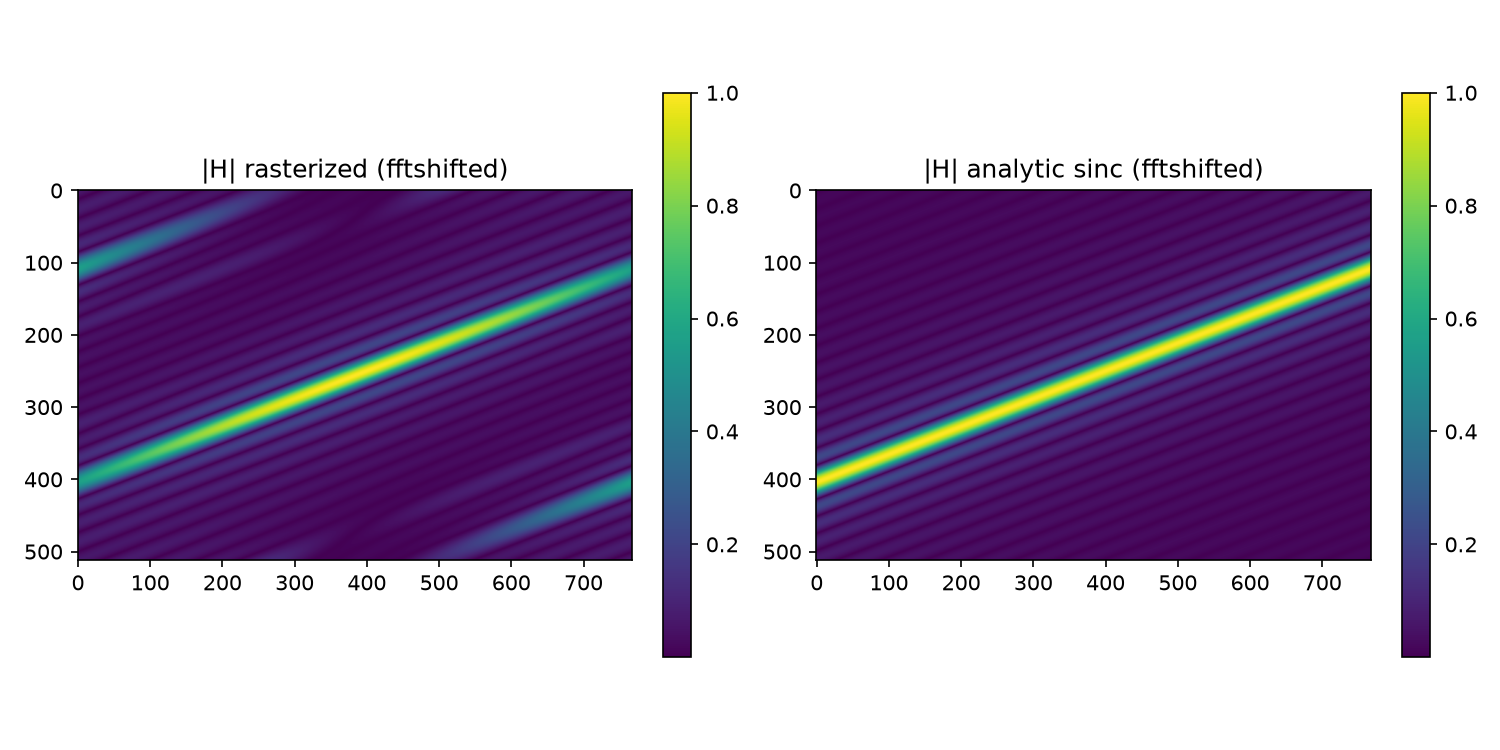
\includegraphics[width=0.8\linewidth]{results/6_1_otf_comparison.png}
\caption{Closed-form analytic OTF versus the DFT of the rasterized spatial kernel. Agreement is
excellent (median $|\Delta H|=0.0136$) except at the Nyquist frequency, where aliasing in the
rasterized kernel is expected to cause disagreement.}
\label{fig:otf_comparison}
\end{figure}

\subsection{Naive inverse filtering}

Table \ref{tab:naive} quantifies the amplification observed at the OTF's near-zero frequencies.

\begin{table}[H]
\centering
\caption{Mean $|\hat F|$ at floored (near-zero-$H$) bins versus other high-frequency bins,
naive inverse filter.}
\label{tab:naive}
\begin{tabular}{lr}
\toprule
Bin category & Mean $|\hat F|$ \\
\midrule
Floored bins ($|H|<10^{-3}$) & $1.49\times10^6$ \\
Other high-frequency bins    & $7.26\times10^4$ \\
\midrule
Ratio & $20.5\times$ \\
\bottomrule
\end{tabular}
\end{table}

\begin{figure}[H]
\centering
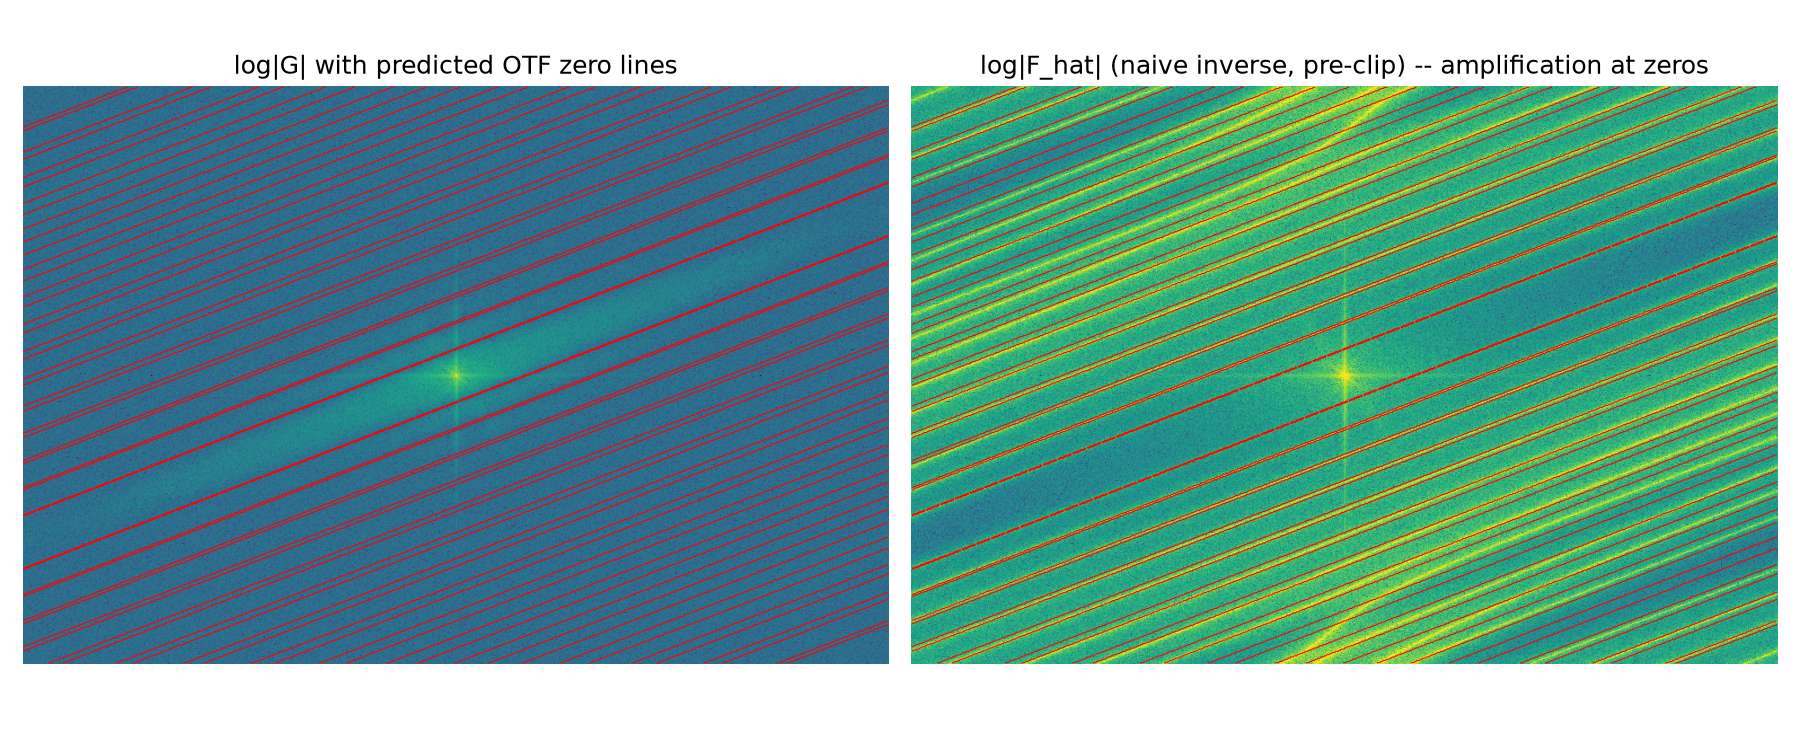
\includegraphics[width=0.8\linewidth]{results/6_2_naive_inverse_spectra.png}
\caption{$\log|G|$ (left) versus the raw, pre-clip naive-inverse spectrum $\log|\hat F|$
(right), with predicted OTF zero lines overlaid in red. Bright streaks in the right panel align
precisely with the predicted zero lines.}
\label{fig:naive_spectra}
\end{figure}

\begin{figure}[H]
\centering
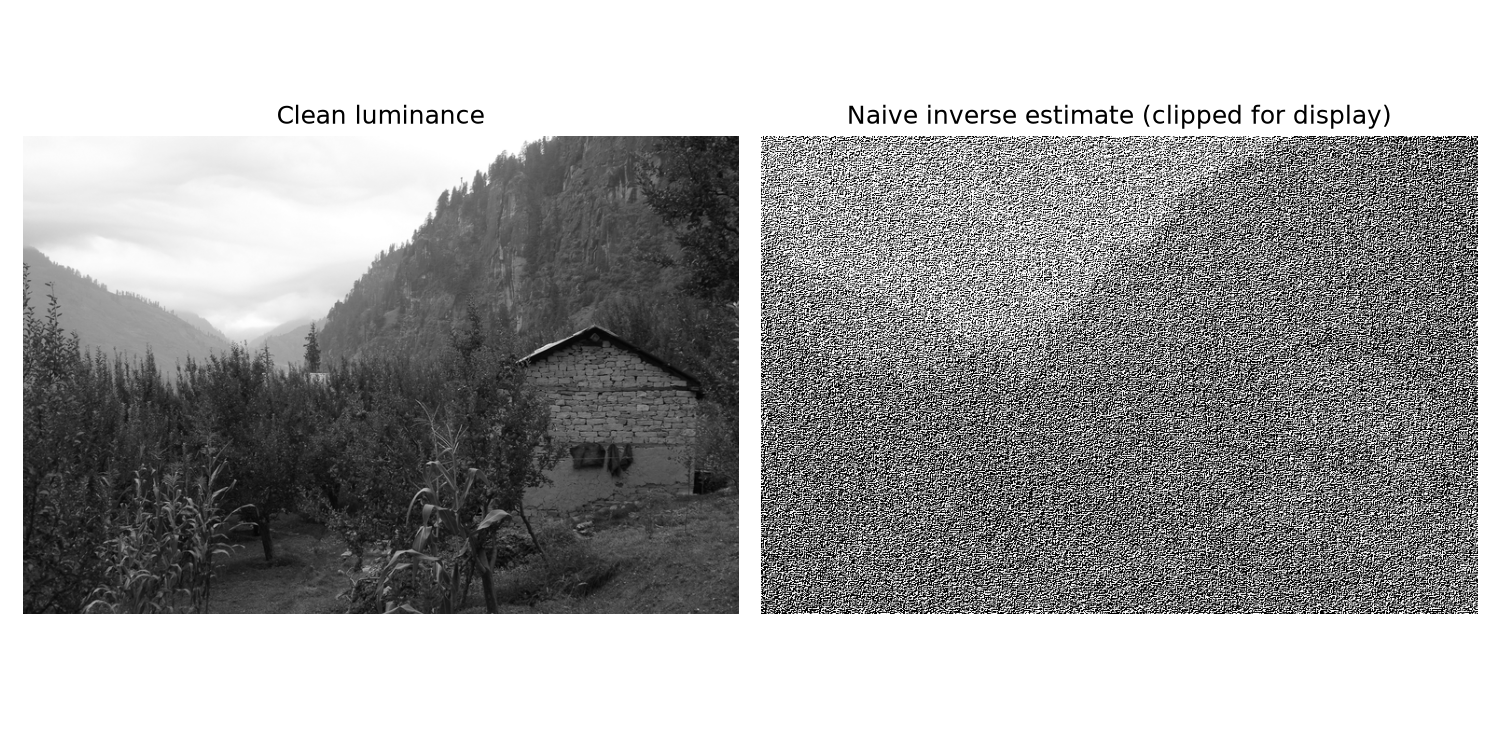
\includegraphics[width=0.6\linewidth]{results/6_2_naive_inverse_image.png}
\caption{Spatial-domain result of the naive inverse filter (display-clipped) — dominated by
amplified noise, since the filter inverts noise just as eagerly as signal at every frequency.}
\label{fig:naive_image}
\end{figure}

As derived in Section 2.3, $\hat F = F + N/H$: wherever $|H|\to0$, a fixed nonzero noise
numerator is divided by a vanishing denominator and diverges without bound, regardless of how
small the actual noise amplitude is — exactly the behaviour quantified above and visible as the
bright streaks precisely overlapping the predicted zero lines.

\subsection{Wiener deconvolution}

Table \ref{tab:ksweep} (from \texttt{results/6\_3\_result.json}) shows the PSNR-optimal $K$ at
each tested SNR level.

\begin{table}[H]
\centering
\caption{Optimal regularization constant $K$ and PSNR achieved, by SNR level.}
\label{tab:ksweep}
\begin{tabular}{lrr}
\toprule
SNR (dB) & Optimal $K$ & PSNR at optimum (dB) \\
\midrule
10 & 0.178   & 18.20 \\
20 & 0.0562  & 21.75 \\
30 & 0.0316  & 24.28 \\
40 & 0.00562 & 26.45 \\
\bottomrule
\end{tabular}
\end{table}

\begin{figure}[H]
\centering
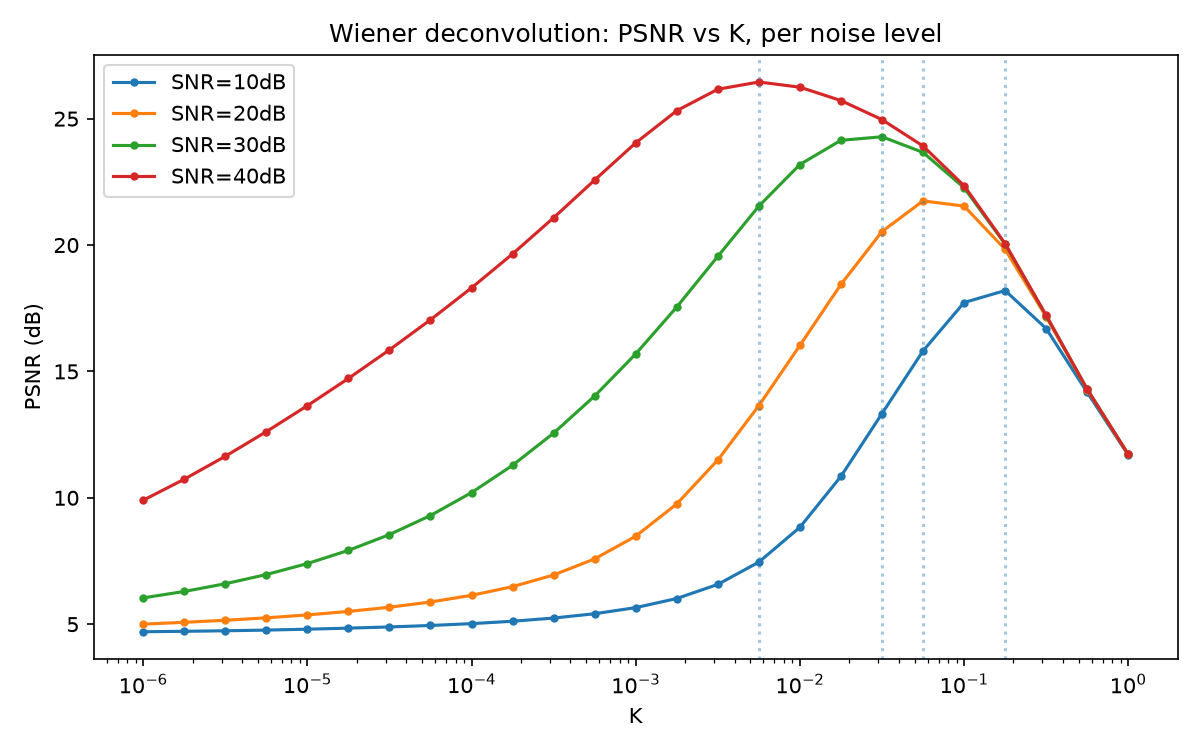
\includegraphics[width=0.8\linewidth]{results/6_3_K_sweep.png}
\caption{PSNR versus regularization constant $K$ at four noise levels; every curve traces a
classic U-shape.}
\label{fig:ksweep}
\end{figure}

\begin{figure}[H]
\centering
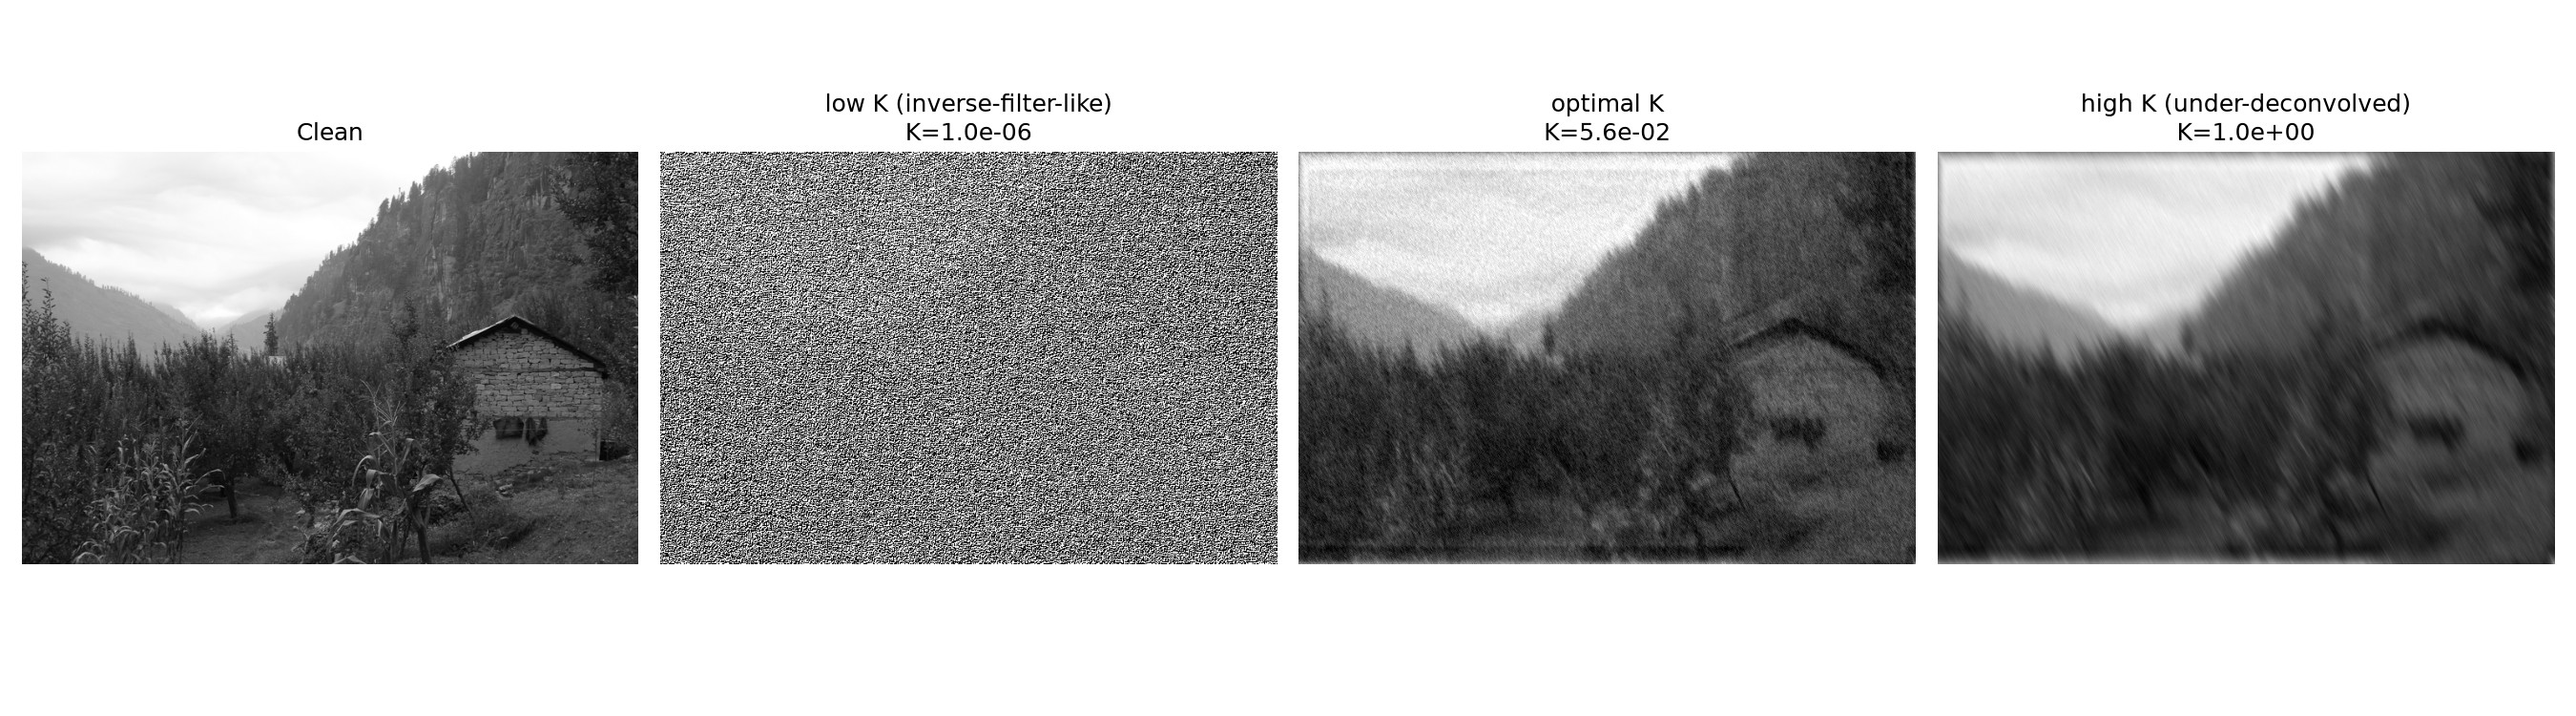
\includegraphics[width=0.8\linewidth]{results/6_3_K_qualitative.png}
\caption{Qualitative Wiener deconvolution output at low, optimal, and high $K$: low $K$
behaves like the naive inverse (noise-dominated); high $K$ under-deconvolves (residual motion
streaking remains visible).}
\label{fig:kqual}
\end{figure}

Every $K$-PSNR curve is a clean U-shape: at low $K$ the filter behaves like the naive inverse
filter (noise amplification dominates, PSNR collapses), while at high $K$ the filter
under-deconvolves (degenerating toward a $H^*/|H|^2$-scaled low-pass response, leaving visible
residual motion blur). The optimal $K$ decreases monotonically as SNR improves (less noise
requires less regularization, so the optimum shifts toward the unregularized inverse filter),
while noisier data needs a larger $K$ to damp the near-zero-OTF amplification identified in
Section 6.2 — exactly the trade-off anticipated by the $K\to0$/$K\to\infty$ limits derived in
Section 2.4.

\subsection{Real motion-blurred photograph: estimation, deconvolution, and model failure}

The blur direction and length were estimated directly from the real photo's own log-magnitude
spectrum (Figure \ref{fig:spectrum}), yielding $\theta_{\mathrm{est}}=99.0^\circ$,
$L_{\mathrm{est}}=2.69$ px, and the image was then Wiener-deconvolved with $K=0.01$
(Figure \ref{fig:real_deblur}).

\begin{figure}[H]
\centering
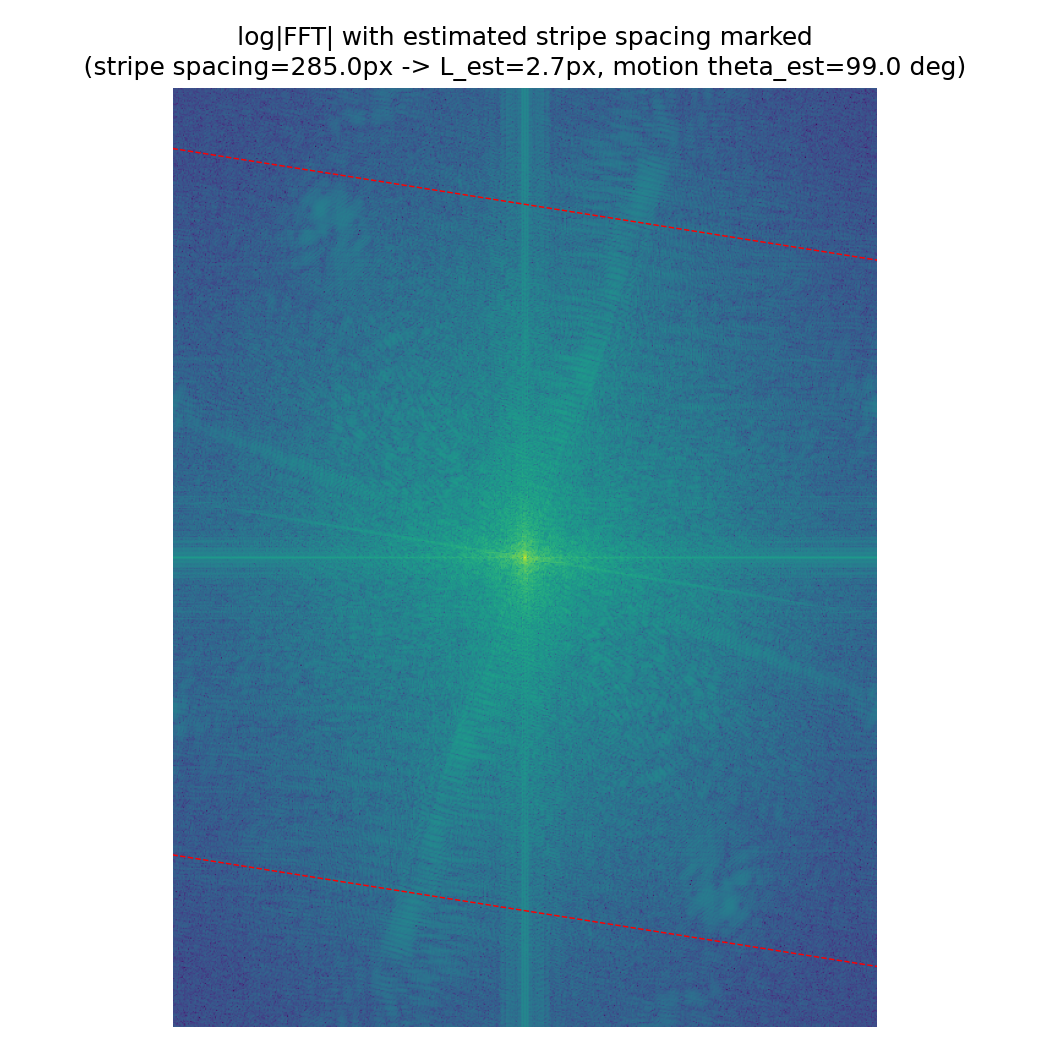
\includegraphics[width=0.7\linewidth]{results/6_4_spectrum_stripes.png}
\caption{The real photo's own log-magnitude spectrum, with the estimated dark-stripe spacing
(perpendicular to $\theta_{\mathrm{est}}$, spaced at the detected 285.0 px period) marked in
dashed red.}
\label{fig:spectrum}
\end{figure}

\begin{figure}[H]
\centering
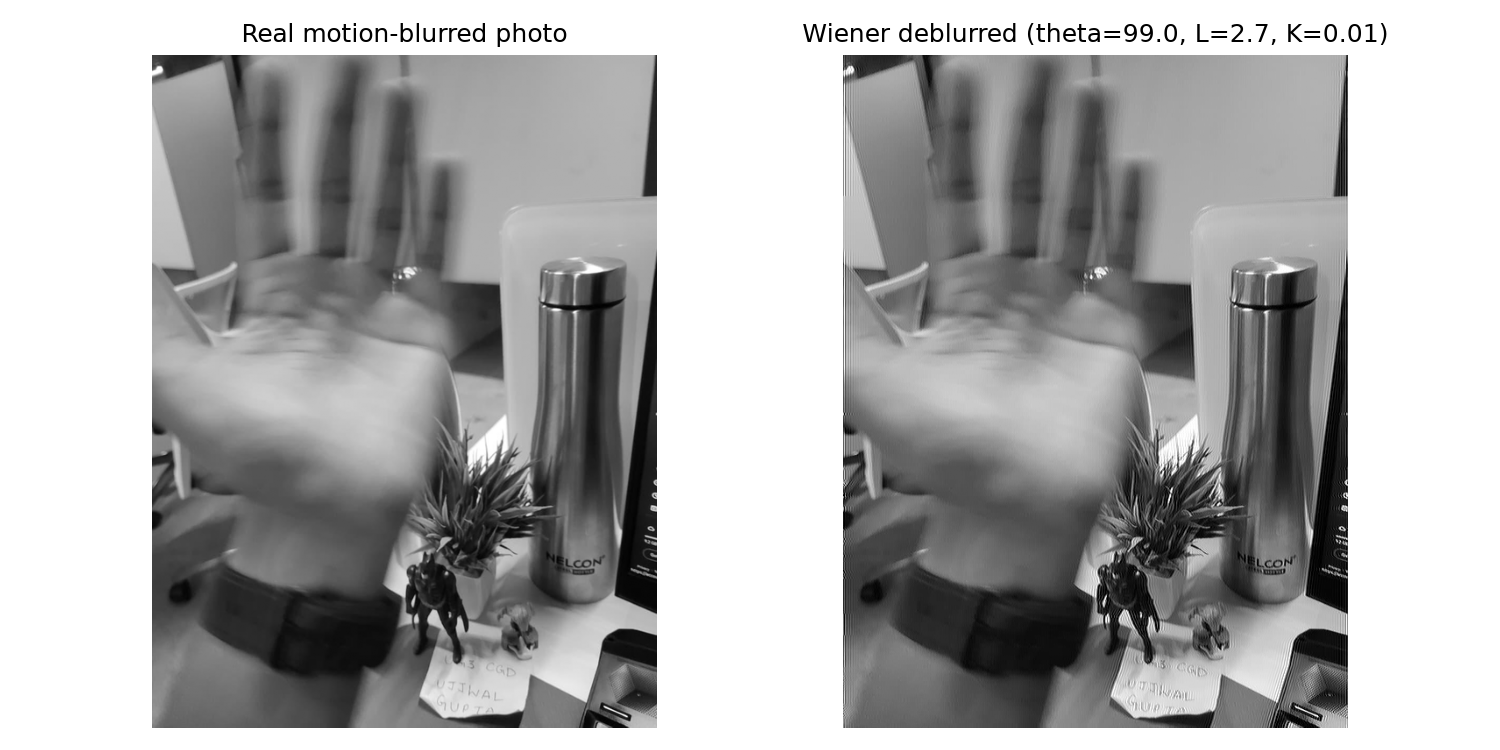
\includegraphics[width=0.7\linewidth]{results/6_4_real_deblur.png}
\caption{Real motion-blurred photograph (hand swiped in front of a stationary desk scene) and
its Wiener-deconvolved result using the estimated $(\theta,L,K)$.}
\label{fig:real_deblur}
\end{figure}

\textbf{This result is itself the required model-failure case study, and is presented honestly
as such rather than hidden.} $L_{\mathrm{est}}\approx2.7$ px is clearly far too small: by eye,
the blur streak on the hand in the original photo spans tens of pixels, not two or three. The
deblurred result confirms this directly — the hand is barely sharpened at all, while the
already-sharp background (the bottle, the chair, the desk edge) instead picks up a faint,
spurious fine vertical ringing/over-sharpening texture: the opposite of a correctly-estimated
deblur.

The failure traces directly to the model's core assumption. The entire linear motion-blur model
of Sections 2.1--2.4 assumes the blur is \textbf{spatially invariant} — the same PSF applies to
every pixel in the frame. In this photo that assumption is badly violated: only the moving hand
is blurred, while the desk, bottle, and background remain sharp. The log-magnitude spectrum used
for estimation is a property of the \emph{whole image at once}, and since most of the frame
(everything except the hand) is sharp, the spectrum is dominated by the sharp background's own
high-frequency content rather than by the comparatively small, localized blur signature from the
hand. The angle-scoring procedure still returns \emph{some} best angle — there is always a
maximum, even a weak or spurious one — but the recovered length is essentially measuring noise
in the mostly-sharp spectrum rather than the true, much larger, localized blur extent.

This is a direct, concrete illustration of exactly the limitation the assignment asks to
identify: a single global $(\theta,L)$ and a single spatially-invariant Wiener deconvolution
cannot correctly handle a photograph where the blur itself varies spatially — here, a moving
\emph{subject} against a stationary background, one of the model's own named failure causes
(alongside camera rotation, changing subject velocity, occlusion, and clipped highlights). A
genuine fix would require first segmenting the moving region and estimating/deconvolving it
locally, entirely outside the single-global-PSF model this problem builds. Evaluated
qualitatively, as required (no clean reference exists for a real photo), the deblurred output is
not a successful deblur of the hand, but it is a correctly diagnosed and clearly explained
failure — arguably the most informative possible outcome for this sub-task, since it makes the
spatially-invariant assumption's real-world fragility directly visible rather than merely stated
in the abstract.

\section{Conclusion}

This problem derived the linear motion-blur PSF as a line integral, its sinc-shaped OTF, and the
perpendicular, $1/L$-spaced geometry of its zero lines; demonstrated concretely why the naive
inverse filter $G/H$ is numerically catastrophic at those zero lines (a $20.5\times$ measured
amplification ratio); derived and implemented the scalar-$K$ regularized Wiener deconvolution
filter as the direct generalization of Problem 5's MMSE denoiser to a known deterministic
degradation, characterizing its $K\to0$/$K\to\infty$ failure limits and confirming the expected
monotonic relationship between optimal $K$ and SNR across four noise levels; and finally applied
the full blind-estimation-plus-deconvolution pipeline to a genuine self-captured motion-blurred
photograph. That final experiment did not produce a visually successful deblur, but produced
something arguably more valuable: a clearly diagnosed, theoretically grounded demonstration that
the spatially-invariant-PSF assumption underlying the entire classical motion-deblurring model
breaks down precisely when it matters most in practice — a localized moving subject against an
otherwise sharp, stationary scene.

\end{document}
